\def\cartesianproductAOneATwo{
    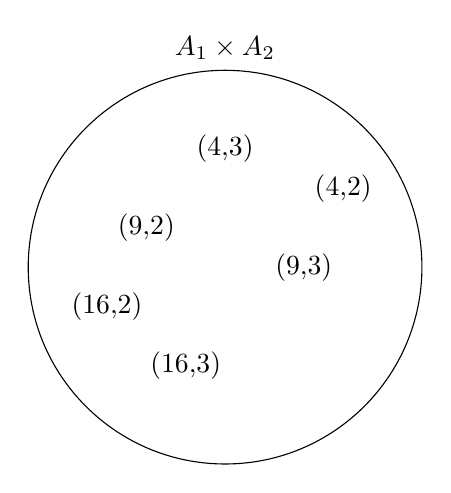
\begin{tikzpicture}
        \node[circle, draw, minimum size=5cm, label=above:{$A_1 \times A_2$}] (set1) at (0,0) {};
        \node at (0,1.5) (P1) {(4,3)};
        \node at (-1,0.5) (P2) {(9,2)};
        \node at (1.5,1) (P3) {(4,2)};
        \node at (1,0) (P4) {(9,3)};
        \node at (-1.5,-0.5) (P5) {(16,2)};
        \node at (-0.5,-1.25) (P6) {(16,3)};
    \end{tikzpicture}
}
\def\cartesianproductRedQ{
    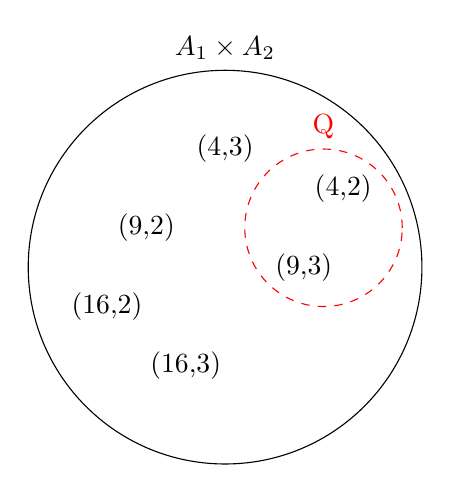
\begin{tikzpicture}
        \node[circle, draw, minimum size=5cm, label=above:{$A_1 \times A_2$}] (set1) at (0,0) {};
        \node at (0,1.5) (P1) {(4,3)};
        \node at (-1,0.5) (P2) {(9,2)};
        \node at (1.5,1) (P3) {(4,2)};
        \node at (1,0) (P4) {(9,3)};
        \node at (-1.5,-0.5) (P5) {(16,2)};
        \node at (-0.5,-1.25) (P6) {(16,3)};
    
        % Dashed red circle around P3 and P4
        \node[circle, draw=red, dashed, minimum size=2cm, label=above:{\textcolor{red}{Q}}] at (1.25,0.5) {};
    \end{tikzpicture}
}
\def\AutomobiliRelationship{
    $Automobili$
        
        \begin{tabular}{|c|c|c|c|c|}
            \hline
            \rowcolor{cyan!30}$Modello$ & $Costruttore$ & $Segmento$ & $Porte$ & $Posti$ \\
            \hline
            Serie 3 & BMW & D & 4 & 5 \\ \hline
            Panda & Fiat & B & 5 & 4 \\ \hline
            Giulietta & Alfa Romeo & C & 5 & 5 \\ \hline
            Bravo & Fiat & C & 5 & 5 \\ \hline
            Punto & Fiat & B & 3 & 5 \\ \hline
            C3 & Citroen & B & 5 & 5 \\ \hline
            C4 & Citroen & C & 5 & 5 \\ \hline
            Delta & Lancia & C & 5 & 5 \\ \hline
        \end{tabular}
}
\begin{frame}{Concetti fondamentali del Modello Relazionale}
Lo sviluppo di un database di un sistema informativo passa attraverso diverse fasi di progettazione, o livelli:
\begin{itemize}[<+->]
    \item livello concettuale;
    \item livello logico;
    \item livello fisico.
\end{itemize}
\pause
\begin{block}{Modello Relazionale}
Il \textbf{modello relazionale} \`e il modello pi\`u utilizzato per la progettazione di basi di dati.
\pause
\newline
\\ In questo modello una base di dati \`e vista come un insieme di tabelle sulle quali possono essere eseguite opportune operazioni.
\pause
\begin{itemize}[<+->]
    \item Il modello \`e chiamato relazionale perch\`e \`e fondato sul concetto matematico di \textbf{relazione} tra insiemi di oggetti.
    \item Esso \`e un modello fondato sui valori.
\end{itemize}
\end{block}
\end{frame}
%
\begin{frame}{Il concetto di Relazione}
Per capire il concetto di relazione e comprendere come si possa rappresentare una relazione mediante tabelle, consideriamo un semplice esempio.

\pause
Consideriamo i 2 insiemi $A_1 = \{4, 9, 16\}$ e $A_2 = \{2, 3\}$.
\pause
\begin{center}
    \begin{tikzpicture}
        \node[circle, draw, minimum size=3.5cm, label=above:{$A_1$}] (set1) at (0,0) {};
        % Label the points in the first set
        \node at (-1,1) (P1) {4};
        \node at (0,0.5) (P2) {9};
        \node at (1,-1) (P3) {16};
    
        \node[circle, draw, minimum size=3.5cm, label=above:{$A_2$}] (set2) at (6,0) {};
        % Label the points in the second set
        \node at (5,1) (A1) {2};
        \node at (6,0.5) (A2) {3};
    \end{tikzpicture}
\end{center}
\end{frame}
%
\begin{frame}{Il concetto di Relazione}
\begin{minipage}[t]{0.4\linewidth}
Prodotto cartesiano tra $A_1$ e $A_2$:
\pause
\begin{center}
\cartesianproductAOneATwo
\end{center}
\end{minipage}%
\hfill%
\begin{minipage}[t]{0.6\linewidth}
\begin{block}{Prodotto cartesiano}
Il \textbf{prodotto cartesiano} di $A_1$ e $A_2$ si indica con $A_1 \times A_2$ ed \`e formato dall'insieme delle coppie $(x,y)$ dove $x$ appartiene ad $A_1$ e $y$ appartiene ad $A_2$.
\end{block}
\end{minipage}
\end{frame}
%
\begin{frame}{Il concetto di Relazione}
\begin{minipage}[t]{0.4\linewidth}
Prodotto cartesiano tra $A_1$ e $A_2$:
\begin{center}
\cartesianproductRedQ
\end{center}
\end{minipage}%
\hfill%
\begin{minipage}[t]{0.6\linewidth}
\begin{block}{Coppie significative}
Alcune coppie del prodotto cartesiano sembrano essere pi\`u significative di altre.
\pause
\\Come per il sottoinsieme $Q$, composo dalle coppie di valori $(x,y)$ dove $x$ \`e il quadrato di $y$.
\pause
\newline
\\ $Q$ pu\`o essere descritto da: ``$x$ \`e il quadrato di $y$'', che esprime la relazione esistente tra $x$ e $y$.
{\scriptsize \[ Q = {(4,2),(9,3)} \subseteq A_1 \times A_2 = {(4,2),(4,3),(9,2),(9,3),(16,2),(16,3)} \]}
\end{block}
\end{minipage}
\end{frame}
%
\begin{frame}{Il concetto di Relazione}
\begin{minipage}[t]{0.4\linewidth}
Prodotto cartesiano tra $A_1$ e $A_2$:
\begin{center}
\cartesianproductRedQ
\end{center}
\end{minipage}%
\hfill%
\begin{minipage}[t]{0.6\linewidth}
\begin{block}{Relazione}
Si dice \textbf{relazione} su due insiemi $A_1$ e $A_2$ un sottoinsieme $R$ del prodotto cartesiano $A_1 \times A_2$.
\end{block}
\pause
\begin{itemize}[<+->]
    \item $Q$ \`e la relazione \textit{QuadratoDi};
    \item Sia $A_1 \times A_2$ che la relazione $Q$, possono essere rappresentate con tabelle!
    \item Ogni tabella \`e composta da tante righe quante sono gli elementi del prodotto cartesiano oppure \textit{QuadratoDi} e da 2 colonne, per rappresentare, ordinatamente, il vlore del primo e del secondo elemento delle coppie $(x,y)$.
\end{itemize}
\end{minipage}
\end{frame}
%
\begin{frame}{Il concetto di Relazione}
\begin{minipage}[t]{0.4\linewidth}
\begin{center}
\cartesianproductRedQ
\end{center}
\end{minipage}%
\hfill%
\begin{minipage}[t]{0.6\linewidth}
\vspace{-5cm}
\begin{center}
    \begin{minipage}{0.4\textwidth}
        \begin{center}
            $A_1 \times A_2$
            
            \pause
            \begin{tabular}{|c|c|}
                \hline
                \rowcolor{cyan!30}$A_1$ & $A_2$ \\
                \hline
                4 & 2 \\ \hline
                4 & 3 \\ \hline
                9 & 2 \\ \hline
                9 & 3 \\ \hline
                16 & 2 \\ \hline
                16 & 3 \\ \hline
            \end{tabular}
        \end{center}
    \end{minipage}
    \hspace{1cm}
    \begin{minipage}{0.4\textwidth}
        \begin{center}
            \pause
            \textit{QuadratoDi}
            \pause
            \begin{tabular}{|c|c|}
                \hline
                \rowcolor{cyan!30}$A_1$ & $A_2$ \\
                \hline
                4 & 2 \\ \hline
                9 & 3 \\ \hline
            \end{tabular}
        \end{center}
    \end{minipage}
\end{center}
\end{minipage}
\end{frame}
%
\begin{frame}{Un esempio concreto di Relazione}
\begin{minipage}{0.9\textwidth}
    Riferendoci al mondo dell'automobile, consideriamo gli insiemi \textit{Modello} e \textit{Costruttore}, cos\`i definiti:
\end{minipage}
\vspace{-.3cm}
\pause
\[ Modello = \{Panda, Cinquecento, C3, C4\}\]
\[ Costruttore = \{Citroen, Fiat\} \]
\begin{minipage}[t]{0.48\linewidth}
\pause
    \begin{center}
        $Modello \times Costruttore$
        
        \pause
        \begin{tabular}{|c|c|}
            \hline
            \rowcolor{cyan!30}$Modello$ & $Costruttore$ \\
            \hline
            Panda & Citroen \\ \hline
            Cinquecento & Citroen \\ \hline
            C3 & Citroen \\ \hline
            C4 & Citroen \\ \hline
            Panda & Fiat \\ \hline
            Cinquecento & Fiat \\ \hline
            C3 & Fiat \\ \hline
            C4 & Fiat \\ \hline
        \end{tabular}
    \end{center}
\end{minipage}%
\hfill%
\begin{minipage}[t]{0.48\linewidth}
    \begin{center}
        \pause
        \textit{ProdottoDa}

        \pause
        \begin{tabular}{|c|c|}
            \hline
            \rowcolor{cyan!30}$Modello$ & $Costruttore$ \\
            \hline
            C3 & Citroen \\ \hline
            C4 & Citroen \\ \hline
            Panda & Fiat \\ \hline
            Cinquecento & Fiat \\ \hline
        \end{tabular}
    \end{center}
\pause
\vspace{-.55cm}
\begin{block}{Nota bene}
    {\small Questo sottoinsieme formato dai 4 elementi di $Modello \times Costruttore$ \`e indicato, \textbf{in modo significativo}, come \textit{ProdottoDa}.}
\end{block}
\end{minipage}
\end{frame}
%
\begin{frame}{Relazione}
Pi\`u in generale:
\begin{block}{Relazione}
Una \textbf{relazione} su $n$ insiemi $A_1, A_2, \ldots, A_n$ \`e un sottoinsieme dell'insieme di tutte le $n$-uple $a_1, a_2, \ldots, a_n$ che si possono costruire prendendo nell'ordine un elemento $a_1$ dal primo insieme $A_1$, $a_2$ dal secondo insieme $A_2$, e cos\`i via.
\pause
\begin{itemize}[<+->]
    \item Una relazione con $n$-colonne si indica come una relazione di \textbf{grado} $n$;
    \item Il nome con il quale si identifica una colonna si chiama \textbf{attributo}.
    \item L'insieme dei valori che possono essere assunti da un attributo definisce il \textbf{dominio} di quell'attributo.
    \item Il numero delle $n$-uple (anche dette tuple) che compongono la tabella si chiama \textbf{cardinalit\`a} della relazione.
\end{itemize}
\end{block}
\end{frame}
%
\begin{frame}{Esempio: grado, cardinalit\`a, attributi e dominio}
\vspace{-.7cm}
\begin{minipage}[t]{0.48\linewidth}
    \begin{center}
        $Modello \times Costruttore$
        
        \begin{tabular}{|c|c|}
            \hline
            \rowcolor{cyan!30}$Modello$ & $Costruttore$ \\
            \hline
            Panda & Citroen \\ \hline
            Cinquecento & Citroen \\ \hline
            C3 & Citroen \\ \hline
            C4 & Citroen \\ \hline
            Panda & Fiat \\ \hline
            Cinquecento & Fiat \\ \hline
            C3 & Fiat \\ \hline
            C4 & Fiat \\ \hline
        \end{tabular}
    \end{center}
\end{minipage}%
\hfill%
\begin{minipage}[t]{0.5\linewidth}
    \begin{center}
        \textit{ProdottoDa}

        \begin{tabular}{|c|c|}
            \hline
            \rowcolor{cyan!30}$Modello$ & $Costruttore$ \\
            \hline
            C3 & Citroen \\ \hline
            C4 & Citroen \\ \hline
            Panda & Fiat \\ \hline
            Cinquecento & Fiat \\ \hline
        \end{tabular}
    \end{center}
\pause
La relazione \textit{ProdottoDa}:
\begin{itemize}
    \item \`e una relazione di \textbf{grado}: \pause 2;
    \item \`e una relazione di \textbf{cardinalit\`a}: \pause 4.
    \item La coppia (Panda, Fiat) \`e una delle 4 tuple della relazione.
\end{itemize}
\end{minipage}
\pause

\vspace{.5cm}
La relazione ha due \textbf{attributi}: \textit{Modello} e \textit{Costruttore} che assumono valori nei 2 domini, formati, rispettivamente, dall'insieme dei modelli di automobili prodotte e dall'insieme dei costruttori di automobili.
\end{frame}
%
\begin{frame}{Esempio: una relazione pi\`u complessa}
\begin{minipage}[t]{0.6\linewidth}
    \begin{center}
        \AutomobiliRelationship
    \end{center}
\end{minipage}%
\hfill%
\begin{minipage}[t]{0.4\linewidth}
\begin{center}
    \begin{itemize}[<+->]
        \item La relazione (o tabella) \textbf{Automobili} rappresenta un'entit\`a;
        \item Ogni $n$-upla rappresenta un'istanza dell'entit\`a;
        \item Le colonne contengono i valori assunti degli attributi dell'entit\`a.
        \item \textbf{Cardinalit\`a}: \pause {8 (numero di tuple/righe/record della tabella);}
        \item \textbf{Grado}: \pause {5 (numero di attributi/colonne/campi della tabella)}.
    \end{itemize}
\end{center}
\end{minipage}
\end{frame}
%
\begin{frame}{Relazioni e chiavi}
\vspace{-.9cm}
\begin{center}
    \AutomobiliRelationship
\end{center}
\pause

L'attributo \textit{Modello} \`e \textbf{chiave} di \textit{Automobili}.

\pause
\begin{block}{Chiave}
    La \textbf{chiave} della relazione \`e un attributo (o una combinazione minimale di attributi) che identifica univocamente le $n$-uple della relazione, cio\`e ogni riga della tabella possiede valori diversi per l'attributo (o gli attributi) chiave.
\end{block}
\end{frame}
%
\begin{frame}{Relazioni e chiavi}
La chiave (formata da uno o pi\`u attributi) identifica la $n$-upla all'interno della tabella:
\pause

per questo motivo il modello relazionale fissa una regola di integrit\`a sui dati, detta\\ \textbf{integrit\`a sull'entit\`a} (entity integrity), secondo cui la chiave primaria non pu\`o avere valore nullo.
\end{frame}
%
\begin{frame}{Rappresentare le tabelle}
Una tabella si rappresenta mediante il suo \textbf{schema}, secondo una struttura del tipo:
\[ \textbf{nomeTabella}(\underline{campoChiave}, campo1, campo2, \ldots, campoN) \]
\pause

identificando tra parentesi, dopo il nome della relazione:
\pause
\begin{itemize}[<+->]
    \item i nomi degli attributi separati dalla virgola;
    \item e sottolineando l'attributo chiave.
\end{itemize}
\pause

\[ \textbf{Automobili}(\underline{Modello}, Costruttore, Segmento, Porte, Posti) \]
\end{frame}
%
\begin{frame}{Rappresentare le tabelle}
Lo \textbf{schema di un database relazionale} \`e definito dallo schema delle tabelle che lo compongono.

\pause

Per esempio, il database con le vendite di prodotti che appartengono a diversi reparti di un negozio, ha il seguente schema:
\[ \textbf{Reparti}(\underline{CodReparto}, NomeReparto) \]
\[ \textbf{Prodotti}(\underline{CodProdotto}, Descrizione, Prezzo, CodReparto) \]
\[ \textbf{Vendite}(\underline{Numero}, Data, Quantita, CodProdotto) \]
\end{frame}